\subsection{Entropia - Fonte Binária}
\begin{frame}%[allowframebreaks]
  \frametitle{Entropia Binária}
  \begin{itemize}
  \item Alfabeto binário $X \in \{0,1\}$, ou $\mathcal{X} = \{0,1\}$.
  \item $p(X=1)=p=1-p(X=0)$.
  \item $H(X) = -p \log p - (1-p) \log (1-p) = H(p)$.
  \item entropia como função de $p$

  \begin{figure}[h!]
  \centering
  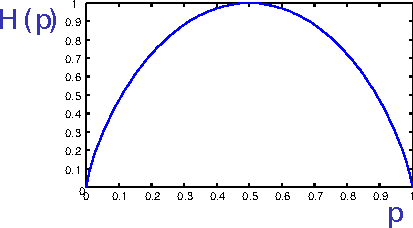
\includegraphics[width=0.5\textwidth]{images/graph_Hp.pdf}
  %\caption{.}
  \label{fig:graph_Hp}
  \end{figure}
  \end{itemize}
\end{frame}
\note{
  \begin{itemize}
  \item maior incerteza ($H=1$) quando $p=0.5$ e menor incerteza ($H=0$) quando $p=0$ ou $p=1$.
  \item note que a entropia $H(p)$ é concava em $p$.
  \end{itemize}
}


\begin{frame}%[allowframebreaks]
  \frametitle{Entropia - GNU Octave}
  \lstinputlisting[firstline=30,lastline=41,label=lst-entropy-fnc]{/home/leoca/ee/research/clscripts/entropy.m}

  \href{https://raw.githubusercontent.com/leolca/clscripts/master/entropy.m}{[download do código]}
\end{frame}

\begin{frame}%[allowframebreaks]
  \frametitle{Entropia - GNU Octave - demo}
  \lstinputlisting[firstline=43,lastline=51,label=lst-entropy-fnc]{/home/leoca/ee/research/clscripts/entropy.m}
\end{frame}

\begin{frame}%[allowframebreaks]
    \frametitle{Entropia - Exemplo}
  Suponha uma v.a. $X \in \mathcal{X} = \{a,b,c,d\}$ com distribuição dada por  
  \begin{equation}
  X = \begin{cases} a, & \text{com probabilidade } \frac{1}{2}, \\
                b, & \text{com probabilidade } \frac{1}{4}, \\
                c, & \text{com probabilidade } \frac{1}{8}, \\
                d, & \text{com probabilidade } \frac{1}{8}.
      \end{cases}
  \end{equation}
  A entropia associada será dada por
  \begin{eqnarray}
   H(X) &=& H\left(\frac{1}{2},\frac{1}{4},\frac{1}{8},\frac{1}{8}\right) = - \sum_{x \in \mathcal{X}} p(x) \log p(x) \nonumber \\
        &=& -\frac{1}{2} \log \frac{1}{2} - \frac{1}{4} \log \frac{1}{4} - \frac{1}{8} \log \frac{1}{8} - \frac{1}{8} \log \frac{1}{8} \nonumber \\
        &=& \frac{1}{2} + \frac{2}{4} + \frac{3}{8} + \frac{3}{8} = \frac{14}{8} = \frac{7}{4} 
  \end{eqnarray}
\end{frame}
